%\begin{figure}[h]
%    \centering
%	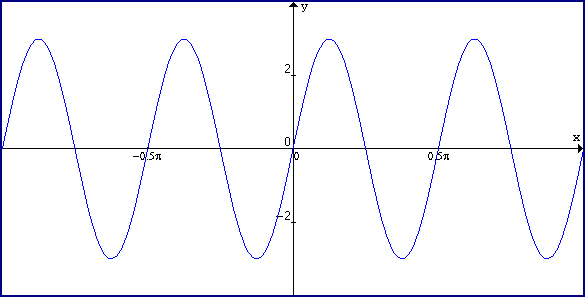
\includegraphics[scale=0.5]{graph}
%	\caption{An example graph}
%	\label{fig:x sine graph}
%\end{figure}

To perform the actual event detection, we propose two algorithms. The first one is a modification of the greedy approach introduced by \cite{event-detection}, which forms events by greedily minimizing temporal and semantical distance of words. We build on top of this algorithm to incorporate the word embeddings as well as alter the temporal distance measure.

The second approach interprets events as literal clusters of words and uses a clustering algorithm to obtain them, rather than explicitly minimize the cost function.

In this chapter, we describe both algorithms, which we will later compare.


\section{Greedy approach}
This algorithm works by grouping word features together by greedily minimizing a cost function representing their temporal and semantic distance. We will first define a distance measure in each of these domains, combine them into the cost function and then describe the algorithm itself.

An event will be represented by a set of keywords. In each iteration, the keyword closest to the event built so far will be added to that event. We will therefore need to measure the distance between a word feature and a whole set of features.

\subsection{Measuring trajectory distance}
After normalization to sum up to 1, the trajectory $\vect{\traj}_{f}$ of a word feature $f$ can be interpreted as a probability distribution over days, with $\traj_{f}(i)$ denoting the probability that a random document published on day $i$ contains $f$. This interpretation allows us to compare the trajectories using information-theoretic techniques, notably the information divergence.

Given a set of word features $\featset$ and another feature $f$ with all trajectories normalized to probabilities, the temporal distance of $f$ to $\featset$ is

\begin{equation}
	\trajdist{\featset}{f} \coloneqq \kl{\vect{\bar{\traj}}_{\featset}}{\vect{\traj}_{f}},
\end{equation}

where $\vect{\bar{\traj}}_{\featset}$ is the mean of all trajectories of features in $\featset$, $\vect{\traj}_{f}$ is the trajectory of feature $f$ and $\kl{\cdot}{\cdot}$ denotes the Kullback-Leibler divergence.


\subsection{Measuring semantic similarity}
Most of the astounding results of the word2vec model come from semantic relations between words being preserved under vector arithmetic, with words concerning the same topic forming clusters. However, as the topic space is high-dimensional, traditional Euclidean distance would vary greatly between different words. Therefore, we use cosine similarity instead, which is bounded in $[-1, 1]$ and independent on the vector lengths. The cosine similarity is a measure often used in information retrieval: \cite{cosine-similarity-i, cosine-similarity-ii}.

Note that we use cosine \textit{similarity} rather than \textit{distance}, which is simply a mean to respect the structure proposed by \cite{event-detection}, who used a simpler measure of document overlap, and the cost function will be constructed accordingly.

Given a set of word features $\featset$ and another feature $f$, the semantic similarity of $f$ and $\featset$ is

\begin{equation}
	\semsim{\featset}{f} \coloneqq \frac{\inp[\big]{\bar{\embed}_{\featset}}{\embed_{j}}}{\| \bar{\embed}_{\featset} \| \cdot \| \embed_{j} \|},
\end{equation}

where $\bar{\embed}_{\featset}$ is the mean of all vector embeddings of features in $\featset$ and $\embed_{f}$ is the vector embedding of the feature $f$. Here, the mean vector is supposed to represent a shared topic among words from $\featset$.


\subsection{Cost function}
Intuitively, an event should be represented by keywords highly correlated in the time domain, concerning the same topic, and with high enough power to be considered representative.

A cost function incorporating all these requirements is therefore defined as

\begin{equation} \label{eq:cost-function}
	\cost{\featset}{f} \coloneqq \frac{\trajdist{\featset}{f}}{\exp(\semsim{\featset}{f}) \cdot \sum_{g \in \featset \cup f}{\text{DPS}_{g}}},
\end{equation}

where we exponentiate the cosine similarity so that the resulting value is always positive. As the algorithm will minimize this function, the resulting events will have low trajectory divergence, high semantic similarity will consist of important keywords.


\subsection{Event detection}
To perform the event detection itself, we mostly adapt the \textit{Unsupervised greedy event detection} algorithm from \cite{event-detection}. We do make a change in the initial sorting and sort the word features in \textit{ascending} rather than descending order. This ensures that words with lower DPS value will get selected first and that the cost function will not be minimized as quickly. As a result, the events will contain more representative keywords. This effectively relaxes the DPS part of the cost function while keeping emphasis on the trajectory distance and semantic similarity.

\begin{algorithm}[H] \label{alg:greedy-event-detection}
\begin{algorithmic}[1]
\caption{Unsupervised greedy event detection}
\Input $\text{Feature set} ~ F = \text{HH or HL}$

\State $\text{Sort the features in ascending DPS order: } DPS_{f_{1}} \leq \dots \leq DPS_{f_{\left\vert F \right\vert}}$

\State $k = 0$

\ForEach{$f \in F$}
	\State $k = k + 1$	
	\State $e_{k} = \{ f \}$
	\State $cost_{e_{k}} = \frac{1}{DPS_{f}}$
	\State $F = F \setminus f$
	
	\While{$F \neq \emptyset$}
		\State $m = \argmin\limits_{m}{\cost{e_{k}}{f_{m}}}$

		\If{$\cost{e_{k}}{f_{m}} < cost_{e_{k}}$}
			\State $cost_{e_{k}} = \cost{e_{k}}{f_{m}}$
			\State $e_{k} = e_{k} \cup f_{m}$
			\State $F = F \setminus f_{m}$
		\Else
			\Break
		\EndIf
	\EndWhile
\EndFor

\Output $\text{Events} ~ \{ e_{1}, e_{2}, \dots, e_{k} \}$
\end{algorithmic}
\end{algorithm}


\section{Cluster-based approach}
This approach uses a clustering algorithm to create clusters out of word features directly, instead of explicitly minimizing a cost function. To achieve this, we need to define a proper distance function, and choose the right clustering algorithm.

\subsection{Distance function}
The distance function used is similar to the cost function in the previous algorithm, except that it is defined pairwise. Since the KL-divergence is not symmetric, we use the Jensen-Shannon divergence instead to measure trajectory distance. The semantic similarity remains unchanged in the form of cosine similarity.

The distance between two word features $f_{i}$,\ $f_{j}$ with trajectories $\vect{\traj}_{i},\ \vect{\traj}_{j}$ and embeddings $\embed_{i},\ \embed_{j}$ is therefore defined as

\begin{equation}
	\distfunc{f_{i}}{f_{j}} \coloneqq \frac{\jsd{\vect{\traj}_{i}}{\vect{\traj}_{j}}}{\exp(\semsim{\embed_{i}}{\embed_{j}})},
\end{equation}

with $\jsd{\vect{p}}{\vect{q}} = \frac{1}{2} \left( \kl{\vect{p}}{\vect{m}} + \kl{\vect{q}}{\vect{m}} \right) ,\ \vect{m} = \frac{1}{2} \left( \vect{p} + \vect{q} \right)$.


\subsection{Clustering algorithm}
We will need to select an appropriate clustering algorithm. The obvious requirement is that the algorithm must not depend on an a priori knowledge of the desired number of clusters. Another requirement is that the algorithm must accept custom distance measures. Speed is not the essence, since the number of representative words is typically in tens to hundreds.

Our experimentation suggests that the best results are obtained using the HDBSCAN algorithm \cite{hdbscan}.

{\color{red} TODO: Describe how that works, including automatic noise detection.}

{\color{blue} TODO: Some comparison of the algorithms tested?}


\subsection{Event detection}
The input and output of the event detection algorithm remains the same as in \ref{alg:greedy-event-detection}, only the internals are different. That makes it easy to swap the two algorithms for comparison.

\begin{algorithm}[H]
\begin{algorithmic}[1]
\caption{Cluster-based event detection}
\Input $\text{Feature set} ~ F = \text{HH or HL}$

\State Precompute a distance matrix $\distmat \in \R^{\left\vert F \right\vert \times \left\vert F \right\vert}$ with $\distmat_{ij} = \distfunc{f_{i}}{f_{j}}$

\State Apply HDBSCAN to $\distmat$, obtaining $k$ clusters and the noisy cluster

\ForEach{$(f, cluster) \in \text{HDBSCAN.clusters}$}
	\If{$cluster \neq noise$}
		\State $e_{cluster} = e_{cluster} \cup f$
	\EndIf
\EndFor

\Output $\text{Events} ~ \{ e_{1}, e_{2}, \dots, e_{k} \}$
\end{algorithmic}
\end{algorithm}
